\documentclass[12pt, t]{beamer}

\usepackage{graphicx}
\usepackage{amsmath}
\usepackage{setspace}
\usepackage{float} 
\usepackage{multido}
\usepackage{multirow}
\usepackage{array}
\usepackage{enumerate}
\usepackage{booktabs}
\usepackage{indentfirst} 
\usepackage[style=mla]{biblatex}
\usepackage{subcaption}
\usepackage{hyperref}
\usepackage{textpos}

\makeatletter
\let\@@magyar@captionfix\relax
\makeatother

\definecolor{Turquoise3}{RGB}{0, 134, 139}
\renewcommand{\emph}[1]{{\color{Turquoise3}\textsl{#1}}}
\newcommand{\C}{\mathbb{C}} \newcommand{\F}{\mathbb{F}} \newcommand{\R}{\mathbb{R}} \newcommand{\Q}{\mathbb{Q}}
\newcommand{\N}{\mathbb{N}}
\newcommand{\myseries}[2]{$#1_1,#1_2,\dots,#1_#2$}
\newcommand{\nullspace}{~\\[15pt]}
\newcommand{\remark}{\textbf{Remark: }}
\newcommand{\scp}[2]{\langle\,#1\,,\,#2\,\rangle} \newcommand{\scpp}{\langle\,\cdot\,,\,\cdot\,\rangle}


\usetheme{Madrid}
\setbeamertemplate{navigation symbols}{}

\addtobeamertemplate{frametitle}{}{
\begin{textblock*}{100mm}(0.85\textwidth,-1cm)

\includegraphics[height=1cm]{logo.png}
\end{textblock*}}

\definecolor{themecolor}{RGB}{25,25,112} 

\usecolortheme[named=themecolor]{structure}

\setbeamertemplate{items}[default]

\hypersetup{
    colorlinks=true,
    linkcolor=themecolor,
    filecolor=themecolor,      
    urlcolor=themecolor,
    citecolor=themecolor,
}

\title{VV285 RC Part I}
\subtitle{\textbf{Elements of Linear Algebra}\\``Matrices are just linear maps!"}
\institute[UM-SJTU JI]{Univerity of Michigan-Shanghai Jiao Tong University Joint Institute}
\author{Xingjian Zhang}

\begin{document}

\begin{frame}
    \titlepage
    \begin{center}
        
\includegraphics[height=2cm]{logo2.png}
    \end{center}
\end{frame}

\begin{frame}
    \frametitle{Something you need to pay attention to...}
    Think More and Be Interactive!
    \begin{itemize}
        \item Do think more about the question in ``()''. \\e.g. ``(How to prove?)''
        \item You are welcome to ask questions in a adequate manner.
        \item Please open your camera so that I can receive more feedbacks from you. (Makes our life easier!) 
        \item The class is designed to be interactive. However, if you really do not want to be asked at all, please type an ``\_'' before your zoom name.
    \end{itemize}
    

\end{frame}

\begin{frame}
    \
    \frametitle{Overview of Linear Algebra}
    \begin{enumerate}
        \item Systems of Linear Equations
        \item Finite-Dimensional Vector Spaces
        \item Inner Product Spaces
        \item Linear Maps
        \item Matrices
        \item Theory of Systems of Linear Equations
        \item Determinants
    \end{enumerate}
\end{frame}

\section{Systems of Linear Equations}
\begin{frame}
    \frametitle{Overview - Systems of Linear Equations}
    \begin{enumerate}
        \item Linear System
              \\ Homogeneous vs. Inhomogeneous
              \\ Underdetermined vs. Overdetermined
        \item Equivalency of Linear System
        \item The Gauß – Jordan Algorithm
        \item Diagonalizable (Existence and Uniqueness of Linear System)
        \item \textbf{Fundamental Lemma for Homogeneous Equations}
    \end{enumerate}
\end{frame}

\subsection{Linear System}
\begin{frame}
    \frametitle{Linear System}

    A \emph{linear system} of $m$ (algebraic) equations in $n$ unknowns \myseries{x}{n}$\in V$ is a set of equations
    \begin{equation}
        \begin{aligned}
            a_{11}x_1+a_{12}x_2+\cdots+a_{1n}x_n & =b_1   \\
            a_{21}x_1+a_{22}x_2+\cdots+a_{2n}x_n & =b_2   \\
                                                 & \vdots \\
            a_{m1}x_1+a_{m2}x_2+\cdots+a_{mn}x_n & =b_m
        \end{aligned}
        \label{eq1}
    \end{equation}

    where \myseries{b}{m}$\in V$ and $a_{ij}\in\F,i=1,\ldots,m,~j=1,\ldots,n.$\\
    If $b_1=b_2=\cdots=b_m=0$, then \eqref{eq1} is called a \emph{homogeneous system}. Otherwise, it is called an \emph{inhomogeneous system.}

    If $m<n$ we say that the system in \emph{underdetermined}, if $m>n$ the system is called \emph{overdetermined}.
    A solution of a linear system of equations \eqref{eq1} is a tuple of elements (\myseries{y}{n})$\in V^n$ such that the predicate \eqref{eq1} becomes a true statement.\\[3pt]
\end{frame}

\subsection{Equivalence of Linear System}
\begin{frame}
    \frametitle{Linear System}
    We say that two systems of linear equations are \emph{equivalent} if any solution
    of the first system is also a solution of the second system and vice-versa.
    Thus the systems
    \begin{equation*}
        \begin{aligned}
            x_1+3x_2-x_3    & =1 \\
            ~~~~~~-5x_2+x_3 & =1 \\
            ~~~~~~10x_2+x_3 & =1
        \end{aligned}
        \qquad\qquad\text{and}\qquad\qquad
        \begin{aligned}
            x_1 & =2 \\x_2&=0\\x_3&=1
        \end{aligned}
    \end{equation*} are \emph{equivalent}.
\end{frame}

\subsection{Gau\ss-Jordan Algorithm}
\begin{frame}
    \frametitle{Gau\ss-Jordan Algorithm}
    The goal of the \emph{Gau\ss-Jordan algorithm} (also called Gau\ss ian elimination) is to transform a system
    \begin{equation*}
        \begin{tabular}{ccc|c}
            $\ast$ & $\ast$ & $\ast$ & $\diamond$ \\
            $\ast$ & $\ast$ & $\ast$ & $\diamond$ \\
            $\ast$ & $\ast$ & $\ast$ & $\diamond$ \\
        \end{tabular}
        \qquad\qquad\qquad\qquad
        \ast\in~\R~or~\C,~~\diamond\in V
    \end{equation*}

    first into the form \\
    \begin{equation}
        \begin{array}{c}
            \begin{tabular}{|ccc|c}
                1 & $\ast$ & $\ast$ & $\diamond$ \\ \cline{1-1}
            \end{tabular} \\
            \begin{tabular}{c|cc|c}
                0 & $1$ & $\ast$ & $\diamond$ \\ \cline{2-2}
            \end{tabular} \\
            \begin{tabular}{cc|c|c}
                0 & $0$ & $1$ & $\diamond$ \\
                \cline{3-3}
            \end{tabular}
        \end{array}
    \end{equation}

    and subsequently into \\
    \begin{equation}
        \begin{array}{c}
            \begin{tabular}{|ccc|c}
                1 & $0$ & $0$ & $\diamond$ \\ \cline{1-1}
            \end{tabular} \\
            \begin{tabular}{c|cc|c}
                0 & $1$ & $0$ & $\diamond$ \\ \cline{2-2}
            \end{tabular} \\
            \begin{tabular}{cc|c|c}
                0 & $0$ & $1$ & $\diamond$ \\
                \cline{3-3}
            \end{tabular}
        \end{array}
    \end{equation}
\end{frame}

\begin{frame}
    \frametitle{Elementary Row Manipulations}
    \textbf{Include:}
    \begin{enumerate}
        \item Swapping (interchanging) two rows,
        \item Multiplying each element in a row with a number,
        \item Adding a multiple of one row to another row.
    \end{enumerate}
    ~\\[15pt]

    \textbf{Result:} Transform a system into a equivalent system.
    Since each row represents an equation, we are essentially \textbf{manipulating equations}.\nullspace

    \textbf{Extension:}
    \href{https://en.wikipedia.org/wiki/Gaussian_elimination\#Applications}{The application of Gau\ss-Jordan Algorithm}
\end{frame}

\begin{frame}
    \frametitle{Exercise}
    \begin{align*}
        x_1-2x_2+3x_3+4x_4 & =2, \\
        x_1-2x_2+5x_3+5x_4 & =3, \\
        -x_1+2x_2-x_3-4x_4 & =2.
    \end{align*}
    In our array notation, this is
    \begin{equation*}
        \begin{array}{cccc|c}
            1  & -2 & 3  & 4  & 2 \\
            1  & -2 & 5  & 5  & 3 \\
            -1 & 2  & -1 & -4 & 2
        \end{array}
    \end{equation*}
    Try to solve this.
\end{frame}

\subsection{Existence and Uniqueness of Solutions}
\begin{frame}
    \frametitle{Solutions of Linear System}
    An inhomogeneous system of equations may have either
    \begin{itemize}
        \item a unique solution or
        \item no solution or
        \item an infinite number of solutions.
    \end{itemize}
    A homogeneous system evidently always has the \emph{trivial solution} \[x_1=x_2=\cdots=x_n=0.\]
    It further either has
    \begin{itemize}
        \item no non-trivial solution or
        \item an infinite number of non-trivial solutions.
    \end{itemize}


\end{frame}

\begin{frame}
    \frametitle{Diagonalization}
    A system of $m$ equations with $n$ unknowns will have a unique solution if and only if it is \emph{diagonalizable}. i.e. It can be transformed into diagonal form.\\[15pt]
    \textbf{Remark:} \emph{Diagonalization} turns out to be an important topic in VV286, especially in terms of \emph{ordinary differential equation systems}.
\end{frame}

\subsection{Fundamental Lemma for Homogeneous Equations}
\begin{frame}
    \frametitle{Fundamental Lemma for Homogeneous Equations}
    The homogeneous system
    \begin{align*}
        a_{11}x_1+a_{12}x_2+\cdots+a_{1n}x_n & =0       \\
                                             & ~~\vdots \\
        a_{m1}x_1+a_{m2}x_2+\cdots+a_{mn}x_n & =0
    \end{align*}
    of $m$ equations in $n$ real or complex unknowns \myseries{x}{n} has a \textbf{non-trivial} solution if $n>m$.\\[15pt]

    \textbf{Remark:} This fundamental lemma contributes to prove that any basis of a vector space has the same length.

\end{frame}

\section{Finite-Dimensional Vector Spaces}

\begin{frame}
    \frametitle{Overview - Finite-Dimensional Vector Spaces}
    \begin{enumerate}
        \item Linear Independence
        \item Span
        \item Basis
        \item Dimension
        \item Basis Extension Theorem
        \item Sum of Vector Space
    \end{enumerate}
\end{frame}

\subsection{Linear Independence}
\begin{frame}
    \frametitle{Linear Independence}
    Let $V$ be a real or complex vector space and \myseries{v}{n}$\in V$. Then the vectors \myseries{v}{n} are said to be \emph{independent} if for all \myseries{\lambda}{n}$\in\F$ \vspace*{-4mm}
    \[\sum_{k=1}^{n}\lambda_kv_k=0\qquad\Rightarrow\qquad\lambda_1=\lambda_2=\cdots=\lambda_n=0.\]

    A finite set $M\subset V$ is called an \emph{independent set} if the elements of $M$ are independent.
    \nullspace
    \remark The definition of linear dependence and the ability to determine whether a subset of vectors in a vector space is linearly dependent are key to determining a basis for a vector space.
\end{frame}

\subsection{Span}
\begin{frame}
    \frametitle{Span}
    Let \myseries{v}{n}$\in V$ and \myseries{\lambda}{n}$\in\F$. Then the expression
    \begin{equation*}
        \sum_{k=1}^{n}\lambda_kv_k=\lambda_1v_1+\cdots+\lambda_nv_n
    \end{equation*}
    is called a \emph{linear combination} of the vectors \myseries{v}{n}. The set
    \[\text{span}\{v_1,\ldots,v_n\}=\left\{y\in V:y=\sum_{k=1}^{n}\lambda_kv_k,\lambda_1,\ldots,\lambda_n\in\F\right\}\]
    is called the \emph{(linear) span} or the \emph{linear hull} of the vectors \myseries{v}{n}.\nullspace
    \textbf{Question: } Does the exponential function $\exp (x)=\sum_{n=0}^{\infty} \frac{x^{n}}{n !}$ belong to the set span $M$ where $M=\left\{f \in C(\mathbb{R}): f(x)=x^{n}, x \in \mathbb{N}\right\} ?$

\end{frame}

\begin{frame}
    \frametitle{Independence $\sim$ Span}
    The vectors \myseries{v}{n}$\in V$ are independent if and only if none of them is contained in the span of all the others.
    \\[15pt]
    (How to prove?)
\end{frame}

\subsection{Basis}
\begin{frame}
    \frametitle{Basis}
    Let $V$ be a real or complex vector space. An $n$-tuple $\mathcal{B}=(b_1,\ldots,b_n)\in V^n$ is called an \emph{(ordered and finite) basis} of $V$
    if every vector $v$ has a \textbf{unique} representation
    \begin{equation}
        v=\sum_{i=1}^{n}\lambda_ib_i,\qquad\qquad\qquad\qquad\lambda_i\in\F.\label{basis}
    \end{equation}
    The numbers $\lambda_i$ are called the \emph{coordinates} of $v$ with respect to $\mathcal{B}$.
    \\[15pt]
    The tuple of vectors (\myseries{e}{n}), $e_i\in\R^n$,
    \begin{equation*}
        e_i=(0,\ldots 0,\mathop{1}_{\begin{subarray}{c}
                \uparrow\\  i\text{th}\\ \text{entry}\end{subarray}},0,\ldots,0),\qquad\qquad i=1,\ldots,n,
    \end{equation*}
    is called the \emph{standard basis} or \emph{canonical basis} of $\R^n$.
\end{frame}

\begin{frame}
    \frametitle{Basis = Independence + Span}
    Let $V$ be a real or complex vector space.\\ An $n$-tuple $\mathcal{B}=(b_1,\ldots,b_n)\in V^n$ is a basis of $V$ if and only if
    \begin{enumerate}
        \item the vectors \myseries{b}{n} are linearly independent, i.e., $\mathcal{B}$ is an independent set,
        \item $V=\text{span}~\mathcal{B}.$
    \end{enumerate}
    (How to prove?)
    \nullspace
    \textbf{Remark:} This theorem is more practical than the definition of basis when proving some set is a basis of some vector space. It helps one decompose the proof into two parts: 1. prove linear independence (uniqueness of \eqref{basis}) 2. prove the span is large enough (existence of \eqref{basis}).
\end{frame}

\begin{frame}
    \frametitle{Exercise}
    Prove or give a counterexample: If $v_1,v_2,v_3,v_4$ is a basis of $V$ and $U$ is a subspace of $V$ such that $v_1,v_2\in U$ and $v_3,v_4\notin U$, then $v_1,v_2$ is a basis of $U$.
    \pause
    \nullspace
    Counterexample: $U=\text{span}\{v_1,v_2,v_3+v_4\}$.


\end{frame}

\subsection{Dimension}
\begin{frame}
    \frametitle{Dimension}
    Let $V$ be a real or complex finite-dimensional vector space, $V\neq\{0\}$. \textbf{Then any basis of $V$ has the same length }(number of elements).
    \nullspace
    \textbf{Remark:} This theorem can be proved by contradiction (Use the definition of basis and the fundamental lemma for homogeneous equations). With such a premise, we can then define the \emph{dimension} of vector space.
    \nullspace
    Let $V$ be a real or complex vector space. Then $V$ is called \emph{finite-dimensional} if either
    \begin{itemize}
        \item $V={0}$ or
        \item $V$ possesses a finite basis.
    \end{itemize}
    If $V$ is not finite-dimensional, we say that it is \emph{infinite-dimensional}.
\end{frame}

\begin{frame}
    \frametitle{Basis Extension Theorem}
    \begin{figure}[H]
        \centering
        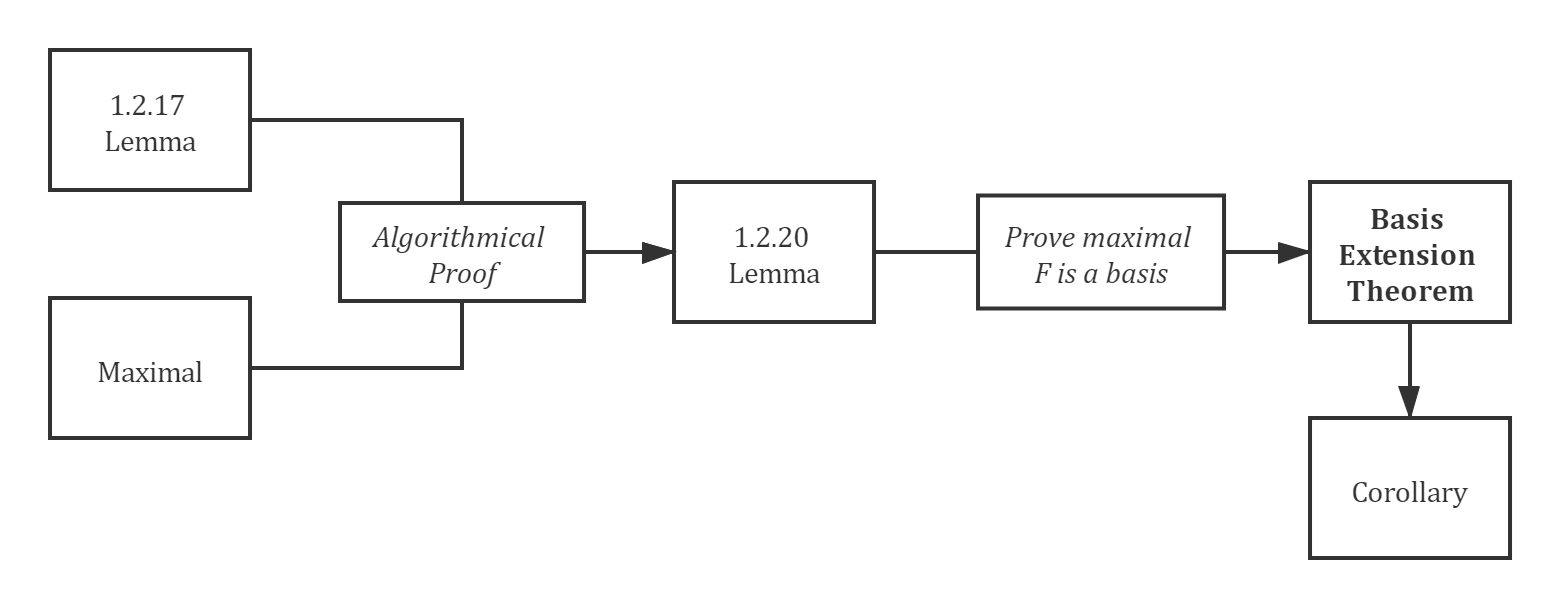
\includegraphics[width=\textwidth]{chart1.png}
        \caption{Logic Flow of Basic Extension Theorem}
        \label{fig:bet}
    \end{figure}
    An interpretation of ``\textbf{maximal}'': the max (in size) independent subset of some set.
\end{frame}

\begin{frame}
    \frametitle{Basis Extension Theorem}
    Let $V$ be a finite-dimensional vector space and $A'\subset V$ an independent set. Then there exists a basis of $V$ containing $A'$.
    \nullspace
    \remark\\
    The basis extension theorem is fundamental. It tells us that for any independent subset $A'$ of a finite-dimensional vector space $V$, we can always find and add dim $V-|A'|$ elements to $A'$ to extend it into a basis of $V$. And two useful corollaries follow immediately:\nullspace
    Let $V$ be an $n$-dimensional vector space, $n\in\N$. Then\\
    \begin{enumerate}
        \item any independent set $A$ with $n$ elements is a basis of $V$.
        \item an independent set $A$ may have at most $n$ elements.
    \end{enumerate}
    (How to prove?)
\end{frame}

\begin{frame}
    \frametitle{Exercise}
    Suppose $p_{0}, p_{1}, \ldots, p_{m}$ are polynomials in $\mathcal{P}_{m}(\F)$ such that $p_{k}(2)=0$ for each $k.$ Prove that $p_{0}, p_{1}, \ldots, p_{m}$ is not linearly independent in $\mathcal{P}_{m}(\F)$

    \pause
    \nullspace
    We express $p_k(x)$ in the form of $p_k(x)=(x-2)q_k(x)$. 
    Immediately, we notice that the degree of $q_k$ is one less than the degree of $p_k$. 
    Therefore, $q_{0}, q_{1}, \ldots, q_{m}$ are polynomials in $\mathcal{P}_{m-1}(\F)$, which has a dimension of $m$. 
    By Corollary 2 we conclude that $q_{0}, q_{1}, \ldots, q_{m}$ are linearly dependent. Correspondingly, $p_{0}, p_{1}, \ldots, p_{m}$ are linearly dependent. 

\end{frame}

\begin{frame}[allowframebreaks]
    \frametitle{Sum of Vector Space}
    Let $V$ be a real or complex vector space and $U,W$ be sets in $V$.
    \begin{enumerate}[(i)]
        \item We define the \emph{sum of U and W} by
              \[U+W:=\left\{v\in V:\mathop{\exists}_{u\in U}\mathop{\exists}_{w\in W}: v=u+w\right\}.\]
        \item If $U$ and $W$ are subspaces of $V$ with $U\cap W=\{0\}$, the sum $U+W$ is called \emph{direct}, and we denote it by $U\oplus W$.
    \end{enumerate}

    It is easy to see that if $U$,$W$ are subspaces of $V$, then $U + W$ and $U\cap W$ are subspaces of $V$. (How to prove?)
    \begin{figure}[H]
        \centering
        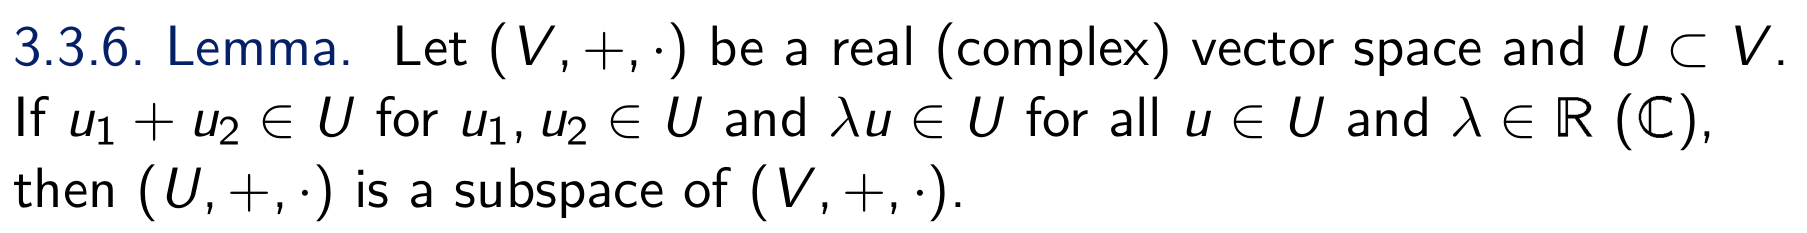
\includegraphics[width=1\textwidth]{2020-05-16-10-31-38.png}
    \end{figure}

    \newpage
    What is the difference between $U+W$ and $U\cup W$?
    \begin{figure}[ht]
        \begin{subfigure}[b]{0.2\textwidth}
            \centering
            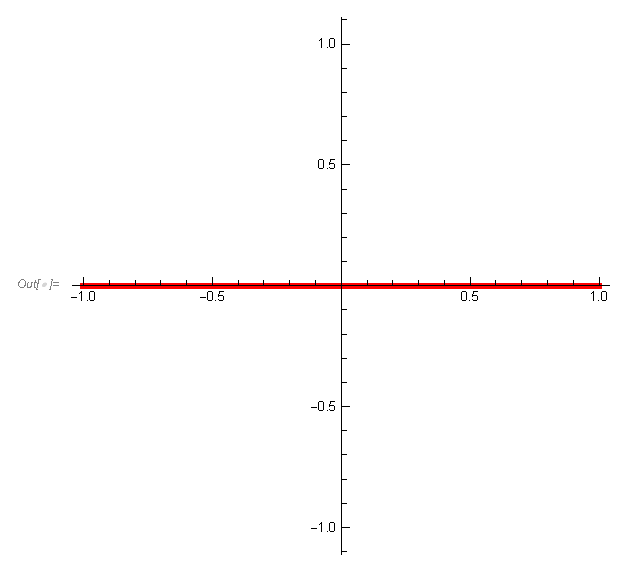
\includegraphics[width=\linewidth]{u+w_gr1.eps}
            \caption{$U$}
        \end{subfigure}
        \begin{subfigure}[b]{0.2\textwidth}
            \centering
            \includegraphics[width=\linewidth]{u+w_gr2.eps}
            \caption{$V$}

        \end{subfigure}
        \begin{subfigure}[b]{0.2\textwidth}
            \centering
            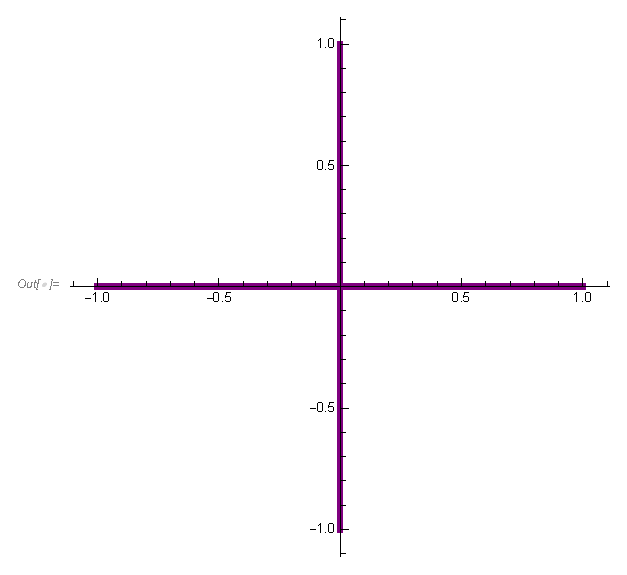
\includegraphics[width=\linewidth]{u+w_gr3.eps}
            \caption{$U\cup V$}
        \end{subfigure}
        \begin{subfigure}[b]{0.2\textwidth}
            \centering
            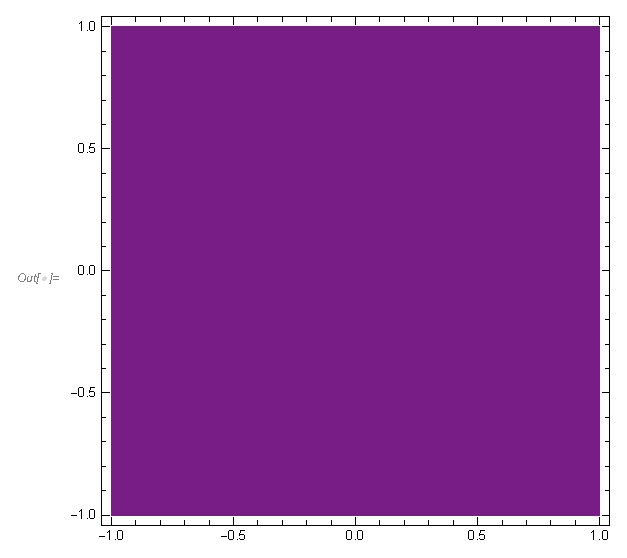
\includegraphics[width=\linewidth]{u+w_gr4.eps}
            \caption{$U+V$}
        \end{subfigure}
    \end{figure}

    \newpage
    Two properties about sum of vector space:\\
    \begin{enumerate}
        \item The sum $U+W$ of vector spaces $U,W$ is direct if and only if all $x\in U+W$, $x\neq0$, have a \textbf{unique} representation $x=u+w,~u\in U,w\in W$.
        \item Let $V$ be a vector space and $U,W\subset V$ be finite-dimensional subspaces of $V$. Then
              \[\dim(U+W)+\dim(U\cap W)=\dim U+\dim W.\]
    \end{enumerate}

\end{frame}

\begin{frame}[allowframebreaks]
    \frametitle{Proof}
    Suppose $$\left\{v_{1}, \ldots, v_{p}\right\}$$ is a basis for $U \cap W$.
    By \emph{Basis Extension Theorem}, we can find a basis
    $$\left\{v_{1}, \ldots, v_{p}, u_{1}, \ldots, u_{q}\right\}$$ for $U$ and a basis
    $$\left\{v_{1}, \ldots, v_{p}, w_{1}, \ldots, w_{r}\right\}$$ for $W$.

    Then we just need to show that $$B=\left\{v_{1}, \ldots, v_{p}, u_{1}, \ldots, u_{q}, w_{1}, \ldots, w_{r}\right\}$$ is a basis for $U+W$\\
    \newpage
    Suppose
    $$
        \alpha_{1} v_{1}+\cdots+\alpha_{p} v_{p}+\beta_{1} u_{1}+\cdots+\beta_{q} u_{q}+\gamma_{1} w_{1}+\cdots+\gamma_{r} w_{r}=0
    $$
    Then
    $$
        x=\underbrace{\alpha_{1} v_{1}+\cdots+\alpha_{p} v_{p}+\beta_{1} u_{1}+\cdots+\beta_{q} u_{q}}_{\in U}=-(\underbrace{\gamma_{1} w_{1}+\cdots+\gamma_{r} w_{r}}_{\in W})
    $$
    belongs to $U \cap W$. Thus
    $$
        x=\delta_{1} v_{1}+\cdots+\delta_{p} v_{p}
    $$
    and therefore
    $$
        \delta_{1} v_{1}+\cdots+\delta_{p} v_{p}=-\left(\gamma_{1} w_{1}+\cdots+\gamma_{r} w_{r}\right)
    $$
    so that
    $$
        \delta_{1} v_{1}+\cdots+\delta_{p} v_{p}+\gamma_{1} w_{1}+\cdots+\gamma_{r} w_{r}=0
    $$
    Since the set $\left\{v_{1}, \ldots, v_{p}, w_{1}, \ldots, w_{r}\right\}$ is linearly independent, we conclude
    $$
        \delta_{1}=0, \quad \ldots, \quad \delta_{p}=0, \quad \gamma_{1}=0, \quad \ldots, \quad \gamma_{r}=0
    $$
    and also that
    $$
        \alpha_{1} v_{1}+\cdots+\alpha_{p} v_{p}+\beta_{1} u_{1}+\cdots+\beta_{q} u_{q}=0
    $$
    So, from linear independence of $\left\{v_{1}, \ldots, v_{p}, u_{1}, \ldots, u_{q}\right\}$ we get
    $$
        \alpha_{1}=0, \quad \ldots, \quad \alpha_{p}=0, \quad \beta_{1}=0, \quad \ldots, \quad \beta_{q}=0
    $$
    Therefore, the set $B$ is independent. It is clear that $\text{span} B=U+W$. So we conclude $B$ is a basis for $U+W$, and furthermore,
    \[\dim(U+W)+\dim(U\cap W)=\dim U+\dim W.\]
\end{frame}

\begin{frame}
    \frametitle{Corollary}
    Let $V$ be a vector space and $U,W\subset V$ be finite-dimensional subspaces of $V$. Then
    \[\dim(U+W)\leq\dim U+\dim W.\]
    The condition for ``='': the sum is direct. i.e.
    \[\dim(U\oplus W)=\dim U+\dim W.\]
\end{frame}

\begin{frame}
    \frametitle{Exercise}
    Suppose that $U=\{(x,x,y,y)\in\F^4:x,y\in\F\}$ and $W=\{(x,x,x,y)\in\F^4:x,y\in\F\}$. Then, what is $U+W$? What is $U\cap W$?
    \pause
    \nullspace
    $$U+W=\{(x,x,y,z)\in\F^4:x,y,z\in\F\}$$
    $$U\cap W=\{(x,x,x,x)\in\F^4:x\in\F\}$$
\end{frame}

\section{Inner Product Spaces}
\begin{frame}
    \frametitle{Overview - Inner Product Spaces}
    \begin{enumerate}
        \item Inner Product Spaces
        \item Induced Norm
        \item Orthogonality \& Orthonormal System
        \item The Projection Theorem
        \item Gram-Schmidt Orthonormalization
    \end{enumerate}

\end{frame}

\subsection{Inner Product Space}
\begin{frame}[allowframebreaks]
    \frametitle{Inner Product Space}
    Let $V$ be a real or complex vector space. Then a map $\langle\,\cdot\,,\,\cdot\,\rangle: V\times V\rightarrow\F$ is called a scalar product or inner product if for all $u,v,w\in V$ and all $\lambda\in\F$
    \begin{enumerate}
        \item \textit{Positive-definite}\\ $\scp{v}{v}\geq0$ and $\scp{v}{v}=0$ if and only if $v=0$,
        \item \textit{Linearity in the 2nd argument}\\ $\scp{u}{v+w}=\scp{u}{v}+\scp{u}{w}$
        \item \textit{Linearity in the 2nd argument}\\ $\scp{u}{\lambda v}=\lambda\scp{u}{v}$
        \item \textit{Conjugate symmetry}\\ $\scp{u}{v}=\overline{\scp{v}{u}}$
    \end{enumerate}
    The pair $(V,\scpp)$ is called an \emph{inner product space}.
    \newpage
    Prove that
    \begin{enumerate}
        \item \[\scp{\lambda u}{v}=\overline{\lambda}\scp{u}{v}.\]
        \item \[\scp{u+v}{w}=\scp{u}{w}+\scp{v}{w}\]
    \end{enumerate}
    This is called the \emph{conjugate linearity} in the 1st argument.
    \nullspace
    What if $\F=\R$?
    \newpage
    What if $\F=\R$?
    \nullspace
    Ans: Conjugate symmetry reduces to symmetry, and conjugate linearity reduces to linearity. So, an inner product on a real vector space is a positive-definite symmetric \emph{bilinear map}.
    \nullspace
    \remark  Multi-linear map will be discussed in detail in \textsl{Differential Calculus - Second Derivative}.

    \newpage
    Why is inner product space important?
    \nullspace
    \begin{itemize}
        \item allow the rigorous introduction of intuitive geometrical notions such as the length of a vector or the angle between two vectors
        \item provide the means of defining orthogonality between vectors (zero inner product)
        \item generalize Euclidean spaces (in which the inner product is the dot product, also known as the scalar product) to vector spaces of any (possibly infinite) dimension, and are studied in functional analysis.
        \item  naturally induces an associated \emph{norm}, thus an inner product space is also a \emph{normed vector space}.
    \end{itemize}
\end{frame}

\subsection{Induced Norm}
\begin{frame}[allowframebreaks]
    \frametitle{Induced Norm}
    Let $(V,\scpp)$ be an inner product space. The map
    \[\|\cdot\|:V\rightarrow\R,\qquad\qquad\|v\|=\sqrt{\scp{v}{v}}\]
    is called the \emph{induced norm} on $V$.
    \nullspace
    (How to prove that an induced norm is actually a norm?)

    \begin{figure}[H]
    \centering
    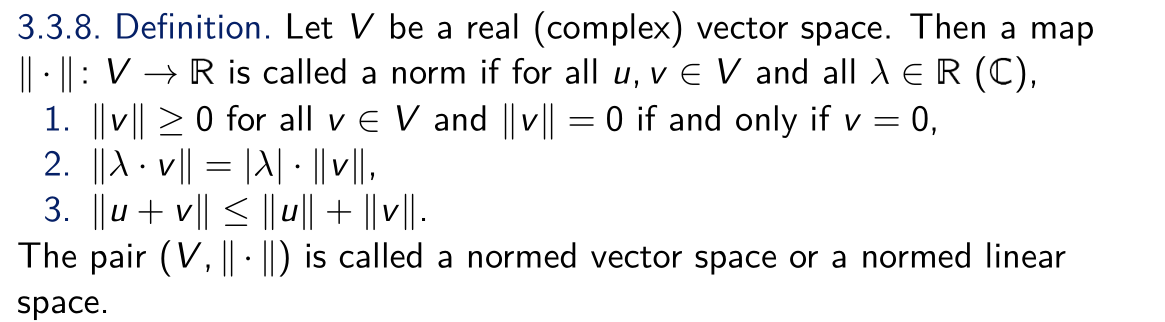
\includegraphics[width=\textwidth]{2020-05-20-13-53-34.png}
    \end{figure}
    
    \newpage
    \begin{itemize}
        \item In $\C^n$ we can define the inner product
            \begin{equation*}
              \scp{x}{y}:=\sum_{i=1}^{n}\overline{x_i}y_i\qquad\qquad
              \qquad x,y\in\C^n.
            \end{equation*}
            \vspace*{-4mm}
        \item In $C([a,b])$, the space of complex-valued, continuous functions on the interval $[a,b]$, we can define an inner product by
            \[\scp{f}{g}:=\int_{a}^{b}\overline{f(x)}g(x)dx,\qquad\qquad
            f,g\in C([a,b]).\]
      \end{itemize}
    \remark Pay attention to the conjugate in two definitions. We will study further on the last one in VV286 to establish \emph{Fourier Series}!

    \newpage
    By \textit{the Cauchy-Schwarz inequality}, we define the \emph{angle} $\alpha(u,v)\in[0,\pi]$ \emph{between u and v} by
    \begin{equation}
        \cos\alpha(u,v)=\frac{\scp{u}{v}}{\|u\|\|v\|}.
    \end{equation}
    We are particularly interested in the case that $\alpha=\pi/2$. i.e. $\scp{u}{v}=0$. Therefore, we introduce \emph{orthogonality}.
\end{frame}

\subsection{Orthogonality}
\begin{frame}[allowframebreaks]
    \frametitle{Orthogonality}
    Let $(V,\scpp)$ be an inner product vector space.
    \begin{enumerate}[1.]
        \item Two vectors $u,v\in V$ are called \emph{orthogonal} or \emph{perpendicular} if $\scp{u}{v}=0$. We then write $u\perp v$.
        \item We call
              \begin{equation*}
                  M^{\perp}:=\left\{v\in V:\mathop{\forall}_{m\in M}\scp{m}{v}=0\right\}
              \end{equation*}
              the \emph{orthogonal complement} of a set $M\subset V$.
    \end{enumerate}
    For short, we sometimes write $v\perp M$ instead of $v\in M^{\perp}$ or $v\perp m$ for all $m\in M$.
    \nullspace
    \remark The orthogonal complement $M^{\perp}$ is a subspace of $V$.\\
    (How to prove?)
\end{frame}

\begin{frame}[allowframebreaks]
    \frametitle{Orthonormal Systems \& Bases}
    Let $(V,\scpp)$ be an inner product vector space. A tuple of vectors (\myseries{v}{r})$\in V$ is called a \emph{(finite) orthonormal system} if
    \begin{equation*}
        \scp{v_j}{v_k}=\delta_{jk}:=\left\{\begin{aligned}&1\;\;\;\text{for }j=k,\\&0\;\;\;\text{for}~j\neq k,\end{aligned}\right.,\qquad\qquad j,k=1,\ldots,r,
    \end{equation*}
    i.e., if $\|v_k\|=1$ and $v_j\perp v_k$ for $j\neq k$.
    \nullspace
    Let $(V,\scpp)$ be a finite-dimensional inner product vector space and $\mathcal{B}=(e_1,\ldots,e_n)$ a basis of $V$. If $\mathcal{B}$ is also an orthonormal system, we say that $\mathcal{B}$ is an \emph{orthonormal basis} (ONB).\\
    \newpage
    \emph{Parseval’s Theorem} Let $(V,\scpp)$ be a finite-dimensional inner product vector space and $\mathcal{B}=\{e_1,\ldots,e_n\}$ an orthonormal basis of $V$. Then
    \begin{equation*}
        \|v\|^2=\sum_{i=1}^{n}|\scp{v}{e_i}|^2
    \end{equation*}
    for any $v\in V$.
    \nullspace
    \remark Parseval’s Theorem gives a alternative way to calculate a vector's induced norm.
\end{frame}

\subsection{Projection Theorem}
\begin{frame}[allowframebreaks]
    \frametitle{Projection Theorem}
    Let $(V,\scpp)$ be a (possibly infinite-dimensional) inner product vector space and (\myseries{e}{r}), $r\in\N$, be an orthonormal system in $V$. Denote $U:=\text{span}\{e_1,\ldots,e_r\}.$\\
    Then for every $v\in V$ there exists a unique representation
    \begin{equation*}
        v=u+w\multido{}{3}{\qquad}\text{where}~u\in U~\text{and}~w\in U^{\perp}
    \end{equation*}
    and $u=\sum\limits_{i=1}^{r}\scp{e_i}{v}e_i,\,w:=v-u.$
    The vector
    \begin{equation*}
        \pi_Uv:=\sum_{i=1}^{r}\scp{e_i}{v}e_i
    \end{equation*}
    is called the \emph{orthogonal projection} of $v$ onto $U$.\\
    \newpage
    The projection theorem essentially states that \textbf{$\pi_Uv$ always exists} and is independent of the choice of the orthonormal system (it depends only on the span $U$ of the system).
    \nullspace
    Moreover, it generalize the idea of projection:
    $$
        \pi_{e_i}v\rightarrow\pi_Uv
    $$
    A vector in an inner product space can be decomposed not only on its \emph{orthonormal basis} but also on its \emph{subspaces}.
\end{frame}

\subsection{Best Approximation}
\begin{frame}
    \frametitle{Orthonormal System $\sim$ Best Approximation}
    \begin{columns}
        \column{0.6\textwidth}
        Why is orthonormal system extremely useful?
        \nullspace
        Let $V$ be a (infinite) vector space. We can approximate an element $v\in V$ using a (finite) linear combination of some orthonormal basis. This is useful in engineering problems.
        \column{0.4\textwidth}
        \begin{figure}[H]
            \centering
            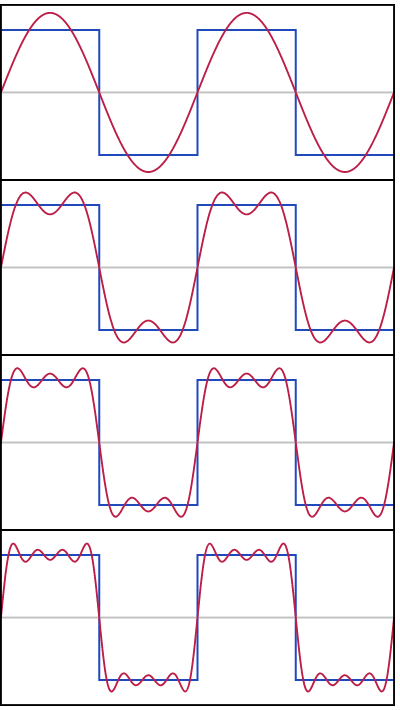
\includegraphics[width=0.6\textwidth]{2020-05-04-01-36-07.png}
            \caption{\small The Fourier Series Approximation of A Square Wave}
        \end{figure}
    \end{columns}
\end{frame}

\begin{frame}
    \frametitle{Gram-Schmidt Orthonormalization}
    Just remember how to do it.
    \begin{align*}
         & w_{1}:=\dfrac{v_{1}}{\left\|v_{1}\right\|}                                                                                                                                                 \\
         & w_{k}:=\dfrac{v_{k}-\sum_{j=1}^{k-1}\left\langle w_{j}, v_{k}\right\rangle w_{j}}{\left\|v_{k}-\sum_{j=1}^{k-1}\left\langle w_{j}, v_{k}\right\rangle w_{j}\right\|}, \quad k=2, \ldots, n
    \end{align*}
    \nullspace
    How to use Gram-Schmidt Orthonormalization to obtain \textit{Legendre polynomials}?
\end{frame}

\begin{frame}
    \frametitle{Discussion}
    \vspace{1.5cm}
    \Large
    \centering
    Learn Well\\
    And\\
    Have Fun!\\


\end{frame}

\end{document}